% This LaTeX was auto-generated from MATLAB code.
% To make changes, update the MATLAB code and export to LaTeX again.

\documentclass{article}

\usepackage[utf8]{inputenc}
\usepackage[T1]{fontenc}
\usepackage{lmodern}
\usepackage{graphicx}
\usepackage{color}
\usepackage{listings}
\usepackage{hyperref}
\usepackage{amsmath}
\usepackage{amsfonts}
\usepackage{epstopdf}
\usepackage{matlab}

\sloppy
\epstopdfsetup{outdir=./}
\graphicspath{ {./ex2018_12_13_IMCL_direct_estimation_single_element_images/} }

\begin{document}

\begin{matlabcode}
syms t(x,d,c)
t(x,d,c) = (sqrt(x^2+d^2)+d)/c
\end{matlabcode}
\begin{matlabsymbolicoutput}
t(x, d, c) = 
    $\displaystyle \frac{d+\sqrt{d^2 +x^2 }}{c}$
\end{matlabsymbolicoutput}
\begin{matlabcode}
assume(-20e-3<=x & x<=20e-3)
assume(1450<=c & c<=1580)
assume(d<=50e-3)
basic_depth = 10e-3;%[m]
basic_sound_speed = 1580;%[m]
freq = 5e6;%[Hz]
syms d(c)
d(c) = basic_depth/basic_sound_speed*c
\end{matlabcode}
\begin{matlabsymbolicoutput}
d(c) = 
    $\displaystyle \frac{934012358162509 c}{147573952589676412928}$
\end{matlabsymbolicoutput}
\begin{matlabcode}
figure;
fplot(t(x,basic_depth,basic_sound_speed)*1e9)%[ns]
xlabel('element position[m]')
ylabel('arrival time[ns]')
hold on
differntial_sound_speed = 1577;
fplot(t(x,d(differntial_sound_speed),differntial_sound_speed)*1e9)%[ns]
xlim([-20e-3 20e-3])
hold off
\end{matlabcode}
\begin{center}
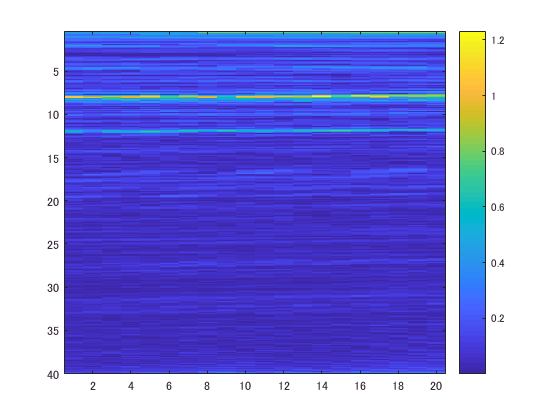
\includegraphics[width=\maxwidth{56.196688409433015em}]{figure_0}
\end{center}
\begin{matlabcode}
figure;
fplot(t(x,d(differntial_sound_speed),differntial_sound_speed)*1e9-t(x,d(basic_sound_speed),basic_sound_speed)*1e9);
xlabel('element position[m]')
ylabel('arrival time[ns]')
xlim([-20e-3 20e-3])
\end{matlabcode}
\begin{center}
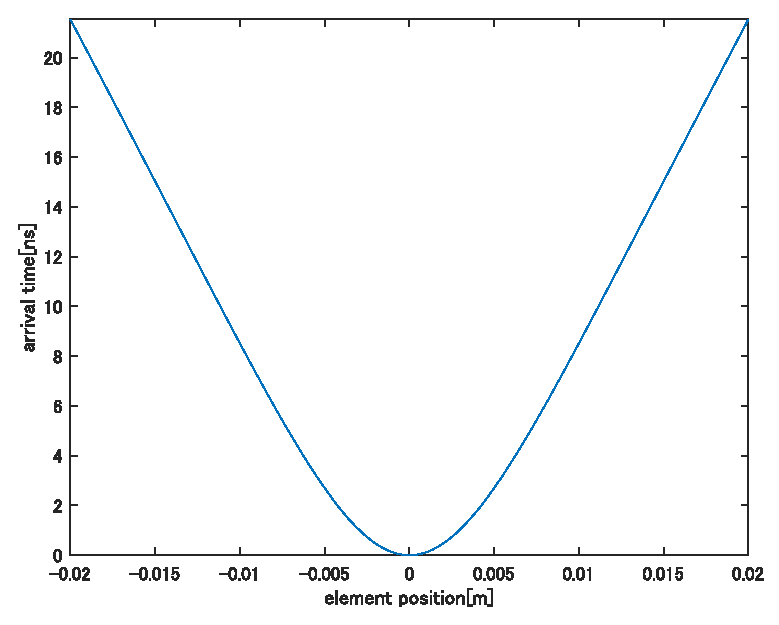
\includegraphics[width=\maxwidth{56.196688409433015em}]{figure_1}
\end{center}
\begin{matlabcode}
1/(freq)*1e9
\end{matlabcode}
\begin{matlaboutput}
ans = 200
\end{matlaboutput}
\begin{matlabcode}
time_36_degree = 1/(freq)*1e9/10
\end{matlabcode}
\begin{matlaboutput}
time_36_degree = 20
\end{matlaboutput}

\begin{par}
\begin{flushleft}
約3 m/sの誤差であれば音速の推定可能性があると考えられる.
\end{flushleft}
\end{par}

\end{document}
